\subsection{EditSQL}

\begin{itemize}
    \item EditSQL focuses on text-to-SQL tasks that are context-dependent across domains.
    \item It exploits the fact that adjacent natural language questions are dependent on one another and that corresponding SQL queries overlap.
    \item To improve the generation quality, they edit the previously predicted query.
    \item The editing mechanism reuses generation results at the token level based on SQL input sequences.
    \item An utterance-table encoder and a table-aware decoder are utilized to incorporate the context of the natural language and the schema when dealing with complicated tables in different domains.
\end{itemize}

\begin{figure}[htb]
    \centering
    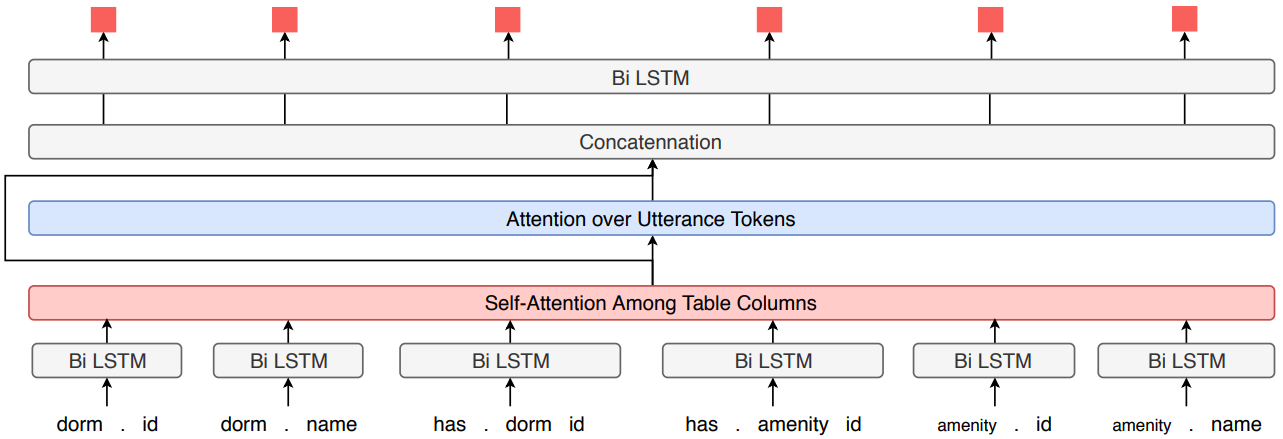
\includegraphics[width=0.8\textwidth]{pics/EditSQL/Table.png}
    \caption{The model architecture of EditSQL from \cite{DBLP:journals/corr/abs-1909-00786}}
    \label{fig:EditSQL}
\end{figure}


\begin{itemize}
    \item User utterances and table schemas are encoded by the utterance-table encoder. Tokens of utterances are encoded using a bi-LSTM.
    \item To determine the most relevant columns, Attention weighed an average of column header embedding is applied to each token.
\end{itemize}

\begin{figure}[htb]
    \centering
    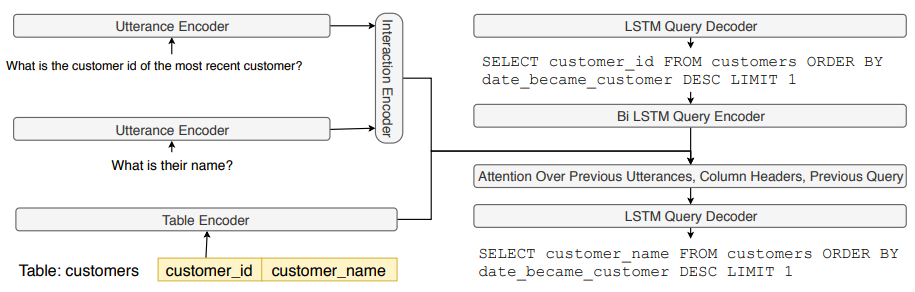
\includegraphics[width=0.8\textwidth]{pics/EditSQL/model.png}
    \caption{An example of user utterance and column headers and Utterance Encoder from \cite{DBLP:journals/corr/abs-1909-00786}}
    \label{fig:EditSQL_model}
\end{figure}

\begin{itemize}
    \item To capture the relationship between table schema and utterance, an attention layer is incorporated.
    \item The utterance-level encoder is built on top of an interaction-level decoder in order to capture information across utterances.
    \item LSTM decoding is used to generate SQL queries by incorporating interaction history, table schema, and user utterances.
\end{itemize}

\begin{figure}[htb]
    \centering
    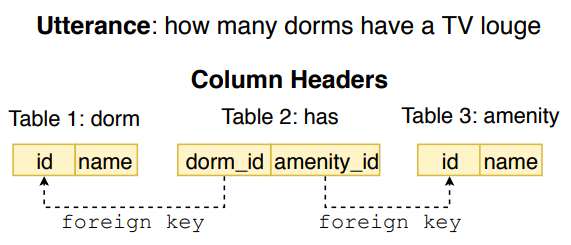
\includegraphics[width=0.5\textwidth]{pics/EditSQL/example.png}
    \caption{Table Encoder from \cite{DBLP:journals/corr/abs-1909-00786}}
    \label{fig:EditSQL_example}
\end{figure}

\begin{itemize}
    \item The model is evaluated on the SParC dataset, a large cross-domain context-dependent semantic parsing dataset derived from SPIDER.
    \item In both SPIDER and SParC, the model outperforms the previous state of the art model, IRNet.
    \item In cross-domain text2SQL generation, the model achieves 32.9\% accuracy. A 53.4\% improvement in accuracy can be achieved by using BERT embedding.
\end{itemize}
